
\chapter{Introduction}

Spoken language\index{spoken language} is one of the most powerful system of communication at our disposal. A large part of our waking hours is spent in social interactions mediated through natural language.  We communicate in order to fulfil a wide array of social functions, such as exchanging ideas, recollecting experiences,  sustaining relationships, or collaborating with others to accomplish shared goals. These communication skills are developed in early childhood, and our cognitive abilities are in many ways shaped and amplified by this disposition for verbal interaction.  This pivotal role of spoken language in our daily lives is largely due to its remarkable efficiency at conveying elaborate thoughts in a robust and effective manner. 

Is it possible to exploit this simple fact to develop more human-friendly technologies? Most of our daily activities are now relying on ``smart'' electronic devices of various kinds, from mobile phones to personal computers and in-car navigation systems. As these technologies gain in autonomy and sophistication, it becomes increasingly important to design appropriate user interfaces\index{user interfaces} that can unlock their full potential.  To be functional, these interface should be made as user-intuitive as possible. In this context, it seems judicious to endow these devices with a capacity to understand, even in a limited manner, the communication medium that is most natural to us, namely spoken language.  

The ongoing research on \textit{spoken dialogue systems}\index{spoken dialogue dystems} (SDS) is precisely trying to achieve this objective. A spoken dialogue system is a computer agent that is able to converse with humans through everyday spoken language in order to perform its task(s). Such systems are expected to play an ever-increasing role in our daily interactions with technology. They have a wide range of applications, ranging from phone-based systems for information access and service delivery to voice-enabled software for hand-held devices, navigation assistants, interactive tutoring systems, and (in a not-too-distant future) service robots assisting us in our everyday environments.

Figure \ref{fig:basicsds} illustrates an example of interaction between a human user and a spoken dialogue system. When the user starts talking, the system extracts the corresponding speech signal through a microphone.  The speech signal is then processed to understand its content.  Once this operation is completed, the system must then decide how to react.  In our case, the system decides to greet back the user and finds the words to express it (\utt{good morning, sir}). The final step is then to synthesise these words through an artificial voice, which closes the loop\footnote{ Needless to say, the schema hides a great deal of internal complexity.  In particular, it omits the existence of non-verbal inputs and outputs (e.g. additional modalities, external actions) which are present in most applications.  The next chapter will describe in more details the software architectures used to design spoken dialogue systems.}.

\begin{figure}[h]
\center
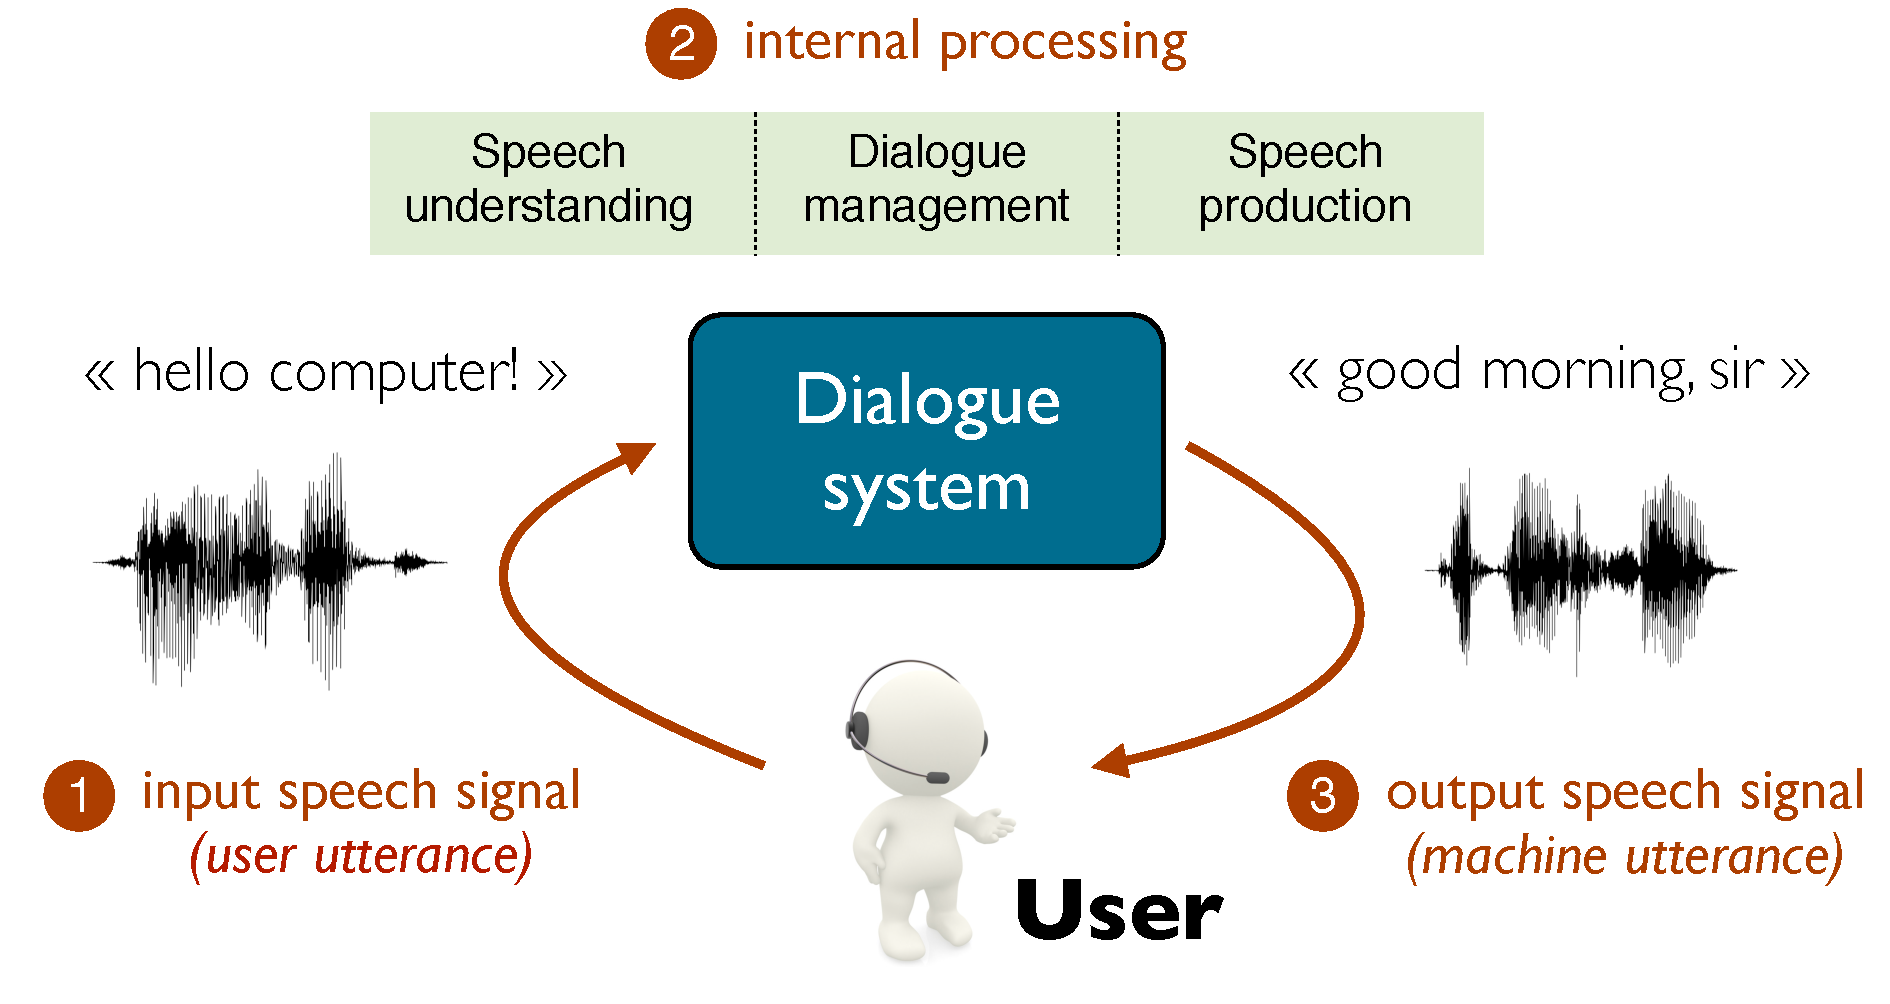
\includegraphics[scale=0.45]{imgs/basicsds.pdf}
\caption{Schematic view of a spoken dialogue system}
\label{fig:basicsds}
\end{figure}

\section{Motivation}

Although the deployment of spoken dialogue systems is attractive for many reasons, their practical development can be a demanding enterprise. Speech is indeed much more complex than other modalities for user interaction such as keyboards or touch screens.  

The present thesis concentrates in particular on the problem of \textit{dialogue management}\index{dialogue management}.  Dialogue management is a central function in spoken dialogue systems.  It serves a double role. 
Its first task is to maintain a representation of the current dialogue state\index{dialogue state}. This representation might include any information that is relevant for the system, and often include features related to the dialogue history, the external context, and the current tasks to perform.  This dialogue state is regularly updated with new information, which comes either in the form of new user utterances or changes in the context. The second task of dialogue management is to make decisions.  Based on the current state of the interaction, dialogue management must decide which actions to undertake. These actions are often communicative in nature (e.g. uttering a sentence), but can also pertain to physical actions to execute (e.g. grasping an object). 

Dialogue management is therefore responsible for controlling the flow of the interaction, by (1) deciding how to interpret the user inputs in their context and (2) selecting which actions to perform next. In the example from Figure \ref{fig:basicsds}, this step corresponds to the decision of responding to the user utterance \utt{hi robot!} with another greeting action \utt{good morning, sir}. 

Dialogue management is a difficult task. To understand why this is the case, it is useful to recall two defining properties of verbal interactions:
\begin{enumerate}
\item Verbal interactions are highly \textit{articulated}.  Their analysis reveals the presence of rich relational structures\index{relational structures} straddling the linguistic and extra-linguistic levels. 
In particular, contextual knowledge\index{context} is essential for the interpretation of most utterances. This is especially the case for conversational domains, where the contributions of the different speakers are built on top of one another in a rapid sequence. A dialogue move is therefore only intelligible within the larger pragmatic context that gave rise to it. 
\item Verbal interactions are also crippled with \textit{uncertainties}\index{uncertainties}.  In order to make sense of a given utterance, a conversational agent must face numerous sources of uncertainty, including error-prone speech recognition, lexical,  syntactic and referential ambiguities, partially observable environments, and unpredictable interaction dynamics.  
\end{enumerate} 

The combination of these two properties forms an explosive mix.  In order to make sense of the interaction and act appropriately, the system must be able to perform complex reasoning operations in order to interpret the user inputs and plan the best course of action.  And it must do so under high levels of noise and uncertainty, where many pieces of information can contain errors or be missing, ambiguous, or fragmentary. This challenge is known in Artificial Intelligence\index{Artificial Intelligence} as \textit{sequential decision-making under uncertainty}\index{sequential decision-making under uncertainty} \citep{aima2010}, and it remains to this day a difficult computational task, especially for complex domains such as spoken dialogue. 

These two challenges mentioned above have typically been addressed in separate lines of research.  On the one hand, structural complexity is often dealt with conceptual tools borrowed from formal logic\index{formal logic}.  These approaches provide principled methods for the interpretation and generation of dialogue moves through logical reasoning on the basis of the inferred beliefs, desires and intentions\index{Belief-Desire-Intention model} of the dialogue participants \citep{Allen1980}. These approaches can provide detailed analyses of various dialogue behaviours, but they generally assume complete observability of the dialogue context and provide only a very limited account (if any) of errors and uncertainties. In addition, they require the knowledge base on which the inference is grounded to be completely specified in advance by domain experts.  Their deployment in practical applications is therefore non trivial. 

On the other hand, the problem of uncertainty is usually addressed by probabilistic modelling\index{probabilistic modelling} techniques.  The state of the dialogue is here represented as a probability distribution over possible worlds.  This distribution represents the system's knowledge of the interaction and is regularly updated as new observations are collected. These probabilistic models provide an explicit account for the various uncertainties that can arise during the interaction. They also enable the dialogue behaviour to be automatically optimised in a data-driven manner instead of relying on hand-crafted mechanisms.  However, these models typically depend on large amounts of training data to estimate their parameters -- a requirement that is hard to satisfy for most dialogue domains.  In addition, the probabilistic models are usually limited to a handful of state variables and are difficult to scale to domains featuring rich conversational contexts. 

The work described in this thesis aims at reconciling these two strands of research with a new computational framework for dialogue modelling. 

\section{Contributions}

The present thesis details a new, hybrid approach to dialogue management based on \textit{structured probabilistic modelling}.  The objective is to design probabilistic models of dialogue that are (1) more scalable to rich domains, (2) easier to estimate from small amounts of training data.

There is an extensive body of work in the machine learning and planning literature which shows how to address this issue by relying on more expressive representations, able to capture relevant aspects of the problem \textit{structure} in a compact manner. By taking advantage of hierarchical or relational abstractions, system developers can leverage their domain knowledge to yield probabilistic models which are both easier to learn (due to a reduced number of parameters) and more efficient to use (since the structure can be exploited by the inference algorithm).

This thesis demonstrates how to translate these insights into dialogue modelling\index{dialogue modelling}. We present a new framework for describing probabilistic models of dialogue, based on the concept of \textit{probabilistic rules}\index{probabilistic rules}.  These rules express the distributions in terms of structured mappings associating specific conditions on a set of input variables to probabilistic effects defined on a set of output variables. 

The presented modelling framework offers two major benefits. Most importantly, the reliance on more expressive representations allows us to drastically reduce the number of parameters associated with the models compared to unstructured approaches.  As a consequence, these models are much easier to learn and to generalise to unseen data. In addition, the framework enables expert knowledge to be directly incorporated into the probabilistic models. System designers are thus free to exploit powerful abstractions to encode their prior knowledge\index{prior knowledge} of the dialogue domain in the form of pragmatic rules, generic background knowledge, or task-specific constraints. 

At runtime, these probabilistic rules are converted into a directed graphical model (a.k.a. a Bayesian Network\index{Bayesian Network}).  The probabilistic rules thus function as high-level templates for a classical probabilistic model.  The resulting Bayesian network is subsequently used to perform various inference operations, e.g. to update the model with new observations or to search for the action yielding the highest utility. These operations are performed via standard algorithms for approximate inference such as importance sampling\index{importance sampling}.

We conducted several experiments to assess the validity of our approach in different learning scenarios: \begin{enumerate}
\item The first experiment, detailed in Section \ref{sec:wozlearning-experiments}, focussed on the problem of estimating the utilities of various system actions given a small data set collected from Wizard-of-Oz interactions\index{Wizard-of-Oz interaction}.\footnote{A Wizard-of-Oz interaction is an experimental procedure borrowed from Human-Computer Interaction (HCI) studies \citep{woz93}. In a Wizard-of-Oz experiment, the subjects are asked to interact with a computer system which has all the appearances of reality, but is actually remotely controlled by an (unseen) human agent operating behind the curtains.  Wizard-of-Oz studies are often conducted to provide the system designers with interaction data from real users before the system is fully implemented.}.  Based on dialogue models encoded with probabilistic rules, the utilities of the different actions were learned through the systematic application of Bayesian inference\index{Bayesian inference} in a supervised learning\index{supervised learning} setting.  We were then able to show that the rule structure enabled the learning algorithm to converge faster and with better generalisation performance than unstructured models. This work was originally presented in \citep{rulebasedmodels-sigdial2012}.
\item The second experiment, described in Section \ref{sec:rllearning-experiments}, extended the above approach to reinforcement learning\index{reinforcement learning}.  In this setting, the parameters are not estimated from gold standards but are gradually learned during the interaction itself, via trial-and-error.  The experiment sought to estimate the transition model of the domain based on a user simulator. We compared the relative learning performance of two modelling approaches: one relying on unstructured distributions, and one based on probabilistic rules. The empirical results demonstrated once more the benefits of capturing the domain structure with probabilistic rules. The results were first published in \note{XXX} 
\item Finally, the third experiment was designed to evaluate the approach through live interactions with real users. \note{to be completed}
\end{enumerate}

An additional contribution of our thesis is a software toolkit that implements all the representations and algorithms presented in this work. The toolkit is called \textsf{openDial}\index{openDial}
 and is freely available under an open source licence.\footnote{The toolkit can be downloaded at \url{http://opendial.googlecode.com}.} \textsf{openDial} allows system developers to design, evaluate and deploy dialogue systems entirely based on probabilistic rules.  The toolkit is fully generic, since all domain-specific knowledge is declaratively specified in the rules for the domain.  This design choice effectively simplifies the system architecture to a small set of core algorithms for accessing and updating the dialogue state \citep{lison-semdial2012}. \textsf{openDial} comes with a user interface allowing developers to interactively test their system and visualise how the internal dialogue state is evolving over time.  The toolkit is described in Appendix \ref{chap:opendial}. 

\begin{wrapfigure}[19]{r}{60mm}
\begin{center}
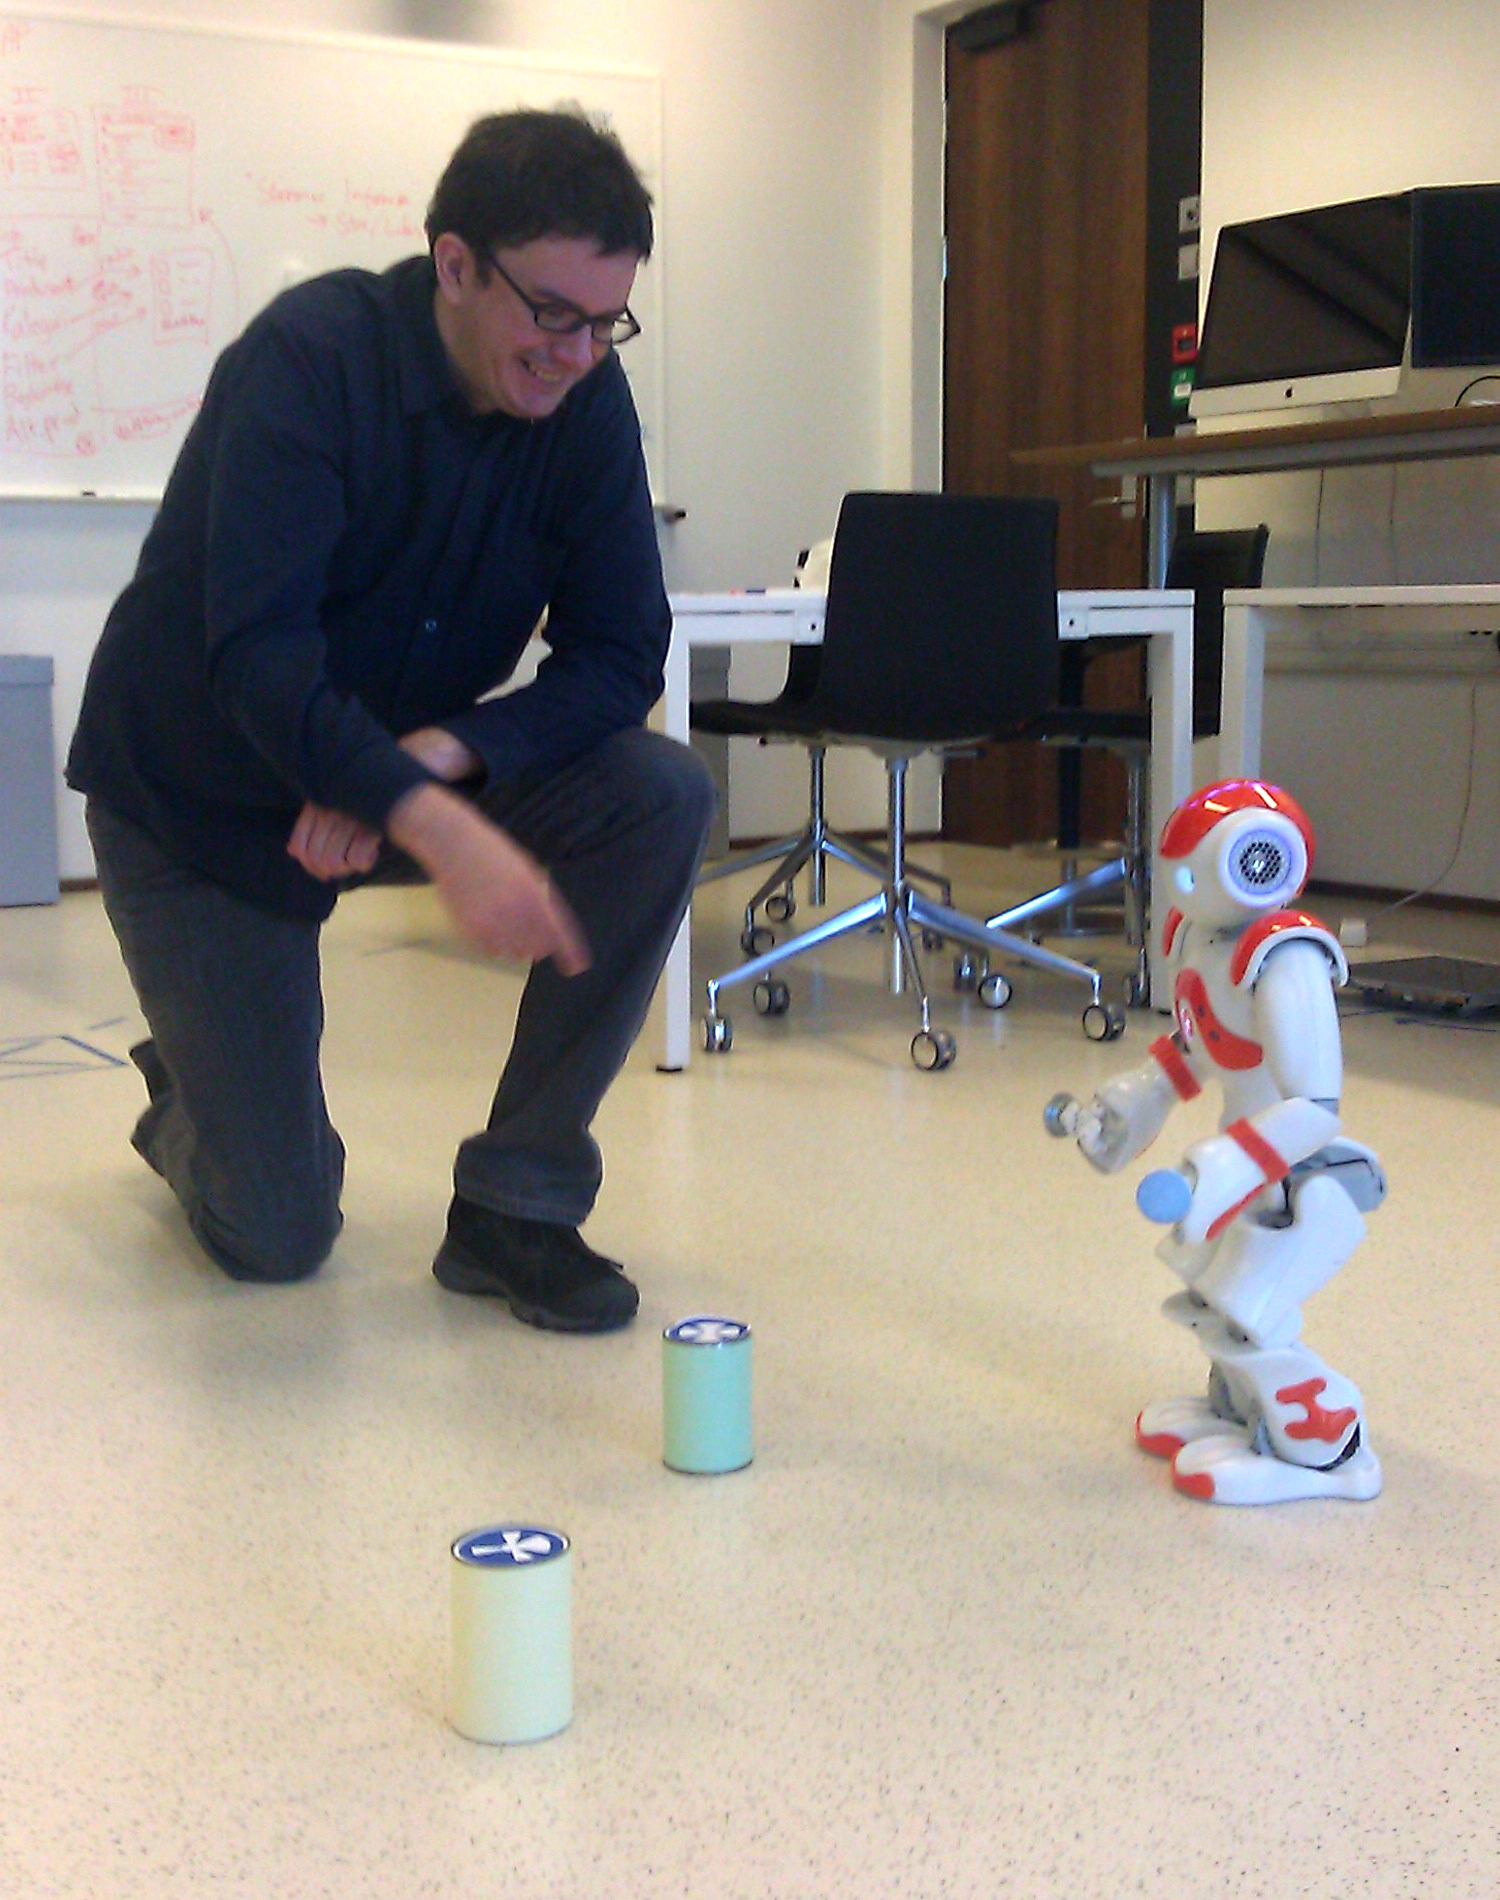
\includegraphics[scale=0.10]{imgs/nao1.jpg}
\end{center} 
\caption{Human user interacting with the Nao robot.}
\label{fig:nao}
\end{wrapfigure}

We conducted all the experiments described in this thesis in a \textit{human--robot interaction} \index{human--robot interaction} (HRI) domain.  The selection of this specific domain as a test bed for our framework was motivated by two factors.  First of all, HRI domains typically embody a rich mix of contextual features extracted from the situated environment and the tasks to complete by the agent. Moreover, HRI domains often have to face significant levels of uncertainty due to imperfect sensors, unreliable motors, and failure-prone speech recognition. 

The Nao robot\index{Nao robot} produced by Aldebaran Robotics was used as a platform for all our experiments \footnote{cf.  \url{http://www.aldebaran-robotics.com}.}.  An example of interaction with the robot is shown in Figure \ref{fig:nao}.  Most of our experiments involved the Nao robot interacting with a human user in a shared visual environment featuring a few basic objects that can be automatically perceived by the robot.  The user were instructed to command the robot to execute various tasks such as grasping objects and moving them from one place to the other.  The robot was also able to answer questions related to his own perception (e.g. \utt{do you see the red cylinder?}).  More details on the exact experimental setup will be provided in the upcoming chapters. 

\section{Outline of the Thesis}

We provide here a brief outline of the thesis structure, chapter by chapter. 
\begin{itemize}
\item \textbf{Chapter \ref{chap:background}} introduces the fundamental concepts and methods used throughout this thesis. We start with an overview of some of the core linguistic properties of dialogue and describe key notions such as turn-taking, dialogue acts and common ground.  We then describe the software architectures that are used to design spoken dialogue systems as well as the role of each individual component.  We also mention a range of important applications for spoken dialogue systems. Finally, we survey the various approaches that have been put forward in the research literature to address the dialogue management problem.  In particular, we review both approaches relying on hand-crafted strategies as well as the more recent statistical approaches.

\item \textbf{Chapter \ref{chap:rules}} lays down the theoretical foundations of our approach.  We start by describing how probabilistic rules are internally structured.  We explain how the rule conditions are expressed and mapped to probabilistic effects.  We also demonstrate how these rules can be used to represent complex probabilistic models. 

We also demonstrate how these rules are instantiated at runtime to update the dialogue state.  

\item \textbf{Chapter \ref{chap:wozlearning}} shows how the parameters attached to probabilistic rules can be automatically learned from training data, in a supervised learning fashion. The algorithm to estimate these parameters is grounded in Bayesian inference.  To validate our approach, we detail an experiment showing how to learn the utilities of a set of actions from Wizard-of-Oz data collected in a human--robot interaction domain.  The experiment illustrates in particular the benefits of applying probabilistic rules.

\item \textbf{Chapter \ref{chap:rllearning}} builds upon the previous chapter and extends it to a reinforcement learning context.  We show that is is possible to learn the parameters of a dialogue model from observations collected during the interaction itself, without having access to any gold standard annotations.  We describe the inner workings of the learning framework, inspired by model-based Bayesian reinforcement learning approaches. The last section details the results of an experiment carried out with a user simulator.  The experiment concentrated on the estimation of the transition model in a HRI domain, and evaluated the relative performance of a  model structured with probabilistic rules compared to a plain probabilistic model.  The empirical results show that, although both models improve their dialogue strategies as more data is collected, the probabilistic rules converge much faster, due to their ability to capture the domain structure in a limited number of parameters.

\item \textbf{Chapter \ref{chap:user-experiments}} 

\end{itemize}